% change according to folder and file names
\ifpdf
    \graphicspath{{4/figures/PNG/}{4/figures/PDF/}{3/figures/}}
\else
    \graphicspath{{4/figures/EPS/}{4/figures/}}
\fi

%: ----------------------- contents from here ------------------------
\chapter{EAs and MAEAs Driven by Principal Component Analysis} % top level followed by section, subsection
\label{VarCorrChapter}
%\begin{flushright}
%Any intelligent fool can make things  
%\linebreak
%bigger, more complex, and more violent. 
%\linebreak
%It takes a touch of genius, and a lot of  
%\linebreak
%courage, to move in the opposite direction.
%\linebreak
%Albert Einstein
%\end{flushright}

This chapter investigates the reasons for the drop in EAs or MAEAs efficiency used to solve ill-posed optimization problems \cite{Salomon,Roy_2002a,Ghisu_2010}, especially when these possess a great number N of design variables, and proposes techniques to overcome this unpleasant situation. Any degradation in the EAs or MAEAs efficiency reflects upon the number of evaluations (on the CFD software, for instance) required to reach the optimal solution(s).  Increasing the number of evaluations leads to longer optimization turn-around times and the routine application of EA-based optimization in large-scale industrial applications is, thus, hindered. The proposed methods adapt the application of the evolution operators accordingly and/or lead to the training of more dependable metamodels on patterns of properly reduced dimension (in case of MAEAs).

Modern industrial-scale optimization problems typically have several objectives and/or constraints with complex parameterization and a great number of design variables. The former is determined by the application under consideration whereas the latter is, often, ``inherited'' from the way experienced designers used to accomplish the same task in the past, without resorting to ``sophisticated'' optimization methods. From the practical point of view, a smooth transition to the EA-based optimization is necessary. Problems with several objectives and/or constraints which handle many design variables can easily become ill-posed, as discussed in section \ref{illpost}. The use of stochastic population-based search methods to solve ill-posed problems leads to excessively long computations, even on modern multi-processor platforms. Since the objectives and constraints are strictly defined by the application, the only way to increase the efficiency of EAs used to solve ill-posed optimization problems is via the appropriate handling of the parameterization. 

Changing the parameterization, though, may have a number of negative effects. First among them is that, in any industrial environment, a valuable amount of experience is embodied into the existing parameterization, in the sense that an experienced designer practically knows qualitatively what to change in order to achieve his/her goal; this would be lost by changing or modifying the parameterization scheme. Also, there is no guarantee that the new/altered parameterization, which must be built in accordance with the objectives so as to give a better-posed optimization problem, includes variables with clear interpretation (being, for instance, the coordinates of \Bezier\ control points, etc.). In fact, this is highly unlikeable. Any new parameterization, with unclear interpretation of the design variables, makes the accumulation of new experience impossible. Furthermore, in a specific project, the best parameterization depends on its correlation with the objectives and constraints. Therefore, a different parameterization would be necessary for any new design-optimization procedure, based on its objectives. To make things even worse, the best parameterization cannot be known in advance, since one should have the Pareto front available (in MOO problems) so as to extract the most appropriate parameterization (see below, in this chapter). All the above can be overcome by implementing the techniques proposed in this chapter.                 


As stated in \cite{Salomon}, standard GAs can find the global optimum in a number of widely used test functions due, not only to the efficiency of the recombination operator and the regular distribution of local minima, but also to the fact that the test functions are decomposable. Though \citep{Salomon} was based on GAs, its outcomes can be generalized to EAs. In \cite{Roy_2002a,Roy_2002b},  it was stated that ``real-life'' engineering design optimisation problems, as opposed to the widely used mathematical test cases, also involve ``interactions among design variables''. There, the notions of ``inseparable function interaction'' and ``variable dependency'' were introduced. The existence  of ``variable dependency'' poses a number of challenges in MOO algorithms which are similar to what is referred to as ill-posed optimization problems.
Also, as stated in \cite{Roy_2002b}, depending upon the nature of ``variable dependency'', additional features such as bias (non-linearity), multi-modality, deception and discontinuity may also occur and these will cause additional loss in the optimization algorithm efficiency. 


%  In \cite{Ghisu_2010}, the merits of adaptive parameterization in MOO with taboo search.



%In the same context with ill-posed optimization problems but with different phrasing significant work has been done by Ralf Salomon, Rajkumar Roy and Tiziano Ghisu. 
%Ralf Salomon presented, in \cite{Salomon}, the efficiency degradation of GAs if the same optimization problem was posed in a ``non-decomposable'' way. Later, Rajkumar Roy presented the, in \cite{Roy_2002a}, the notions of ``Inseparable Function Interaction'' and ``Variable Dependence''. Tiziano Ghisu, in \cite{Ghisu_2010}, presented the merits of adaptive parameterization in MOO with taboo search. 

 

\section{Ill-Posed Optimization Problems}
\label{illpost}
The two main reasons for increasing the number of calls to the evaluation software  required by an EA or MAEA, in order to locate the optimal solution(s), are: (a) the high number of design variables, $N\!>>$ and (b) the fact that an ill-posed optimization problem is solved. Needless to say that a high-dimensional ill-posed optimization problem is the worst case for an EA or MAEA.  Unfortunately, in practice, most engineering optimization problems share both features mentioned above . 

In EAs, the high number of design variables (N) results in efficiency loss. In the best case (well-posed problem), the cost for computing the optimal design(s) increases linearly with N. In MAEAs, the presence of $N\!>>$ design variables, apart from the way the optimal solution is approached (direct effect), impacts also the use of metamodels for which the training time and, mainly, their  prediction error increase noticeably. The loss in efficiency due to the ``less-accurate'' metamodel predictions (indirect effect) is, practically, superimposed to the performance degradation caused by the direct effect.  As a remedy to optimization problems with $N\!>>$, the KBD method was proposed in Chapter 3. From a completely different point of view, the KBD method reduces the problem dimension by exploiting the knowledge embodied into a small number of available archived designs and has already been presented and validated.             

On the other hand, ill-posed optimization problems are those dealing with (a) anisotropic and (b)  non-separable objective function/s $f(\vec{x})$. Note that (a) is a prerequisite for (b). In fact, ill-posed optimization problems are those dealing with non-separable objective functions. The definitions of anisotropic and non-separable functions follow in sections \ref{IllCon} and \ref{Nonsep}, respectively. Ill-posed problems, in combination with $N\!>>$, give rise to the so-called ``curse of dimensionality''. This stands for the situation in which the cost for solving an optimization problem increases superlinearly, instead of just linearly, with N. 
% Thus an ill-post optimization problem, when solved with EAs, is magnifying the negative effects of big N. 

%Herein the definitions of a) anisotropic objective function and b) non-separable objective function that characterize the objective function of an ill-posed problem are presented. Later, an investigation regarding the effects of ill-posed optimization problems on EA efficiency is carried out.  

\subsection{Anisotropic Objective Function}
\label{IllCon}
%The term anisotropic objective function refers to the condition were the contribution to the objective function value is largely anisotropic for the different design variables or ,more precisely, directions in search space.
An objective function $f(\vec{x})$, $\vec{x}=(x_1,...,x_N)$  is anisotropic with respect to $\vec{x}$ if it is differently affected by the same changes in the different components of $\vec{x}$. Though this thesis is dealing with non-gradient-based optimization methods, the anisotropy of f can be quantified by the variation of $\frac{\partial f}{\partial x_i}$ among the design variables $i$, close to the optimal solution. 

%This variation, and thus the magnitude of anisotropy, can be quantified via the condition number (a) of the Hessian matrix (H).


Let as assume that the convex-quadratic objective function
\begin{eqnarray}
   f(\vec{x}) = \frac{1}{2}\vec{x}^TH\vec{x}
   \label{conv.1}
\end{eqnarray}
where $H$ is a symmetric positive definite $N \times N$ matrix.
The variations in $\frac{\partial f}{\partial x_i}$  are expressed by the condition number a of matrix H. In such a case, $a$ is defined as the ratio of H's largest to smallest eigenvalue. 
These two eigenvalues correspond to the squared relative lengths of the principal axes of the ellipsoid $\vec{x}^TH\vec{x}\! =\! 1$. For points located along the principal axes, the gradient aligns with the axis itself and the ellipsoid-axis length determines the magnitude displacement in the design space required for obtaining a certain change in f. Therefore, f is said to be isotropic if the condition number of $H$ is $a=1$ (corresponding to a sphere or hyper-sphere-like isolines, see fig.\ \ref{illc}, left) and anisotropic if $a\!>>\!1$ (corresponding to an ellipse-like isolines, see fig.\ \ref{illc}, right).

  


\begin{figure}[h!]
\begin{minipage}[b]{1.0\linewidth}
 \centering
 \resizebox*{15cm}{!}{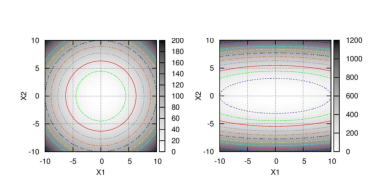
\includegraphics{ellipseA.eps}}
\end{minipage}
%\begin{minipage}[b]{0.5\linewidth}
% \centering
% \resizebox*{7.5cm}{!}{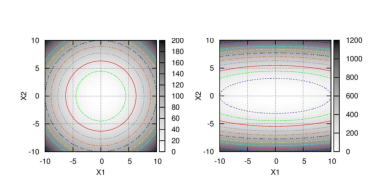
\includegraphics{ellipseA.eps}}
%\end{minipage}
\caption{Iso-value contours of an isotropic objective function with two design variables (left); the impact of $x_1$ and $x_2$ on f is the same. Iso-value contours of an anisotropic objective function, in which $x_2$ has greater impact on f than $x_1$ (right).} 
\label{illc}
\end{figure}

In practice, EAs are capable to efficiently deal with anisotropic objective functions without damaging their efficiency. If, however, the objective function is anisotropic and non-separable (see definition in section \ref{Nonsep}), the EA or MAEA is expected to perform less efficiently, unless a particular treatment is employed; such a treatment is proposed in this chapter.  

Furthermore, the anisotropy of f leads to the notion of more and less important design variables (or, in the case of non-separable f, more and less important directions in the design space). This piece of information can be used to reduce N, via the truncation of less important variables during the metamodel training phase, so as to increase its prediction ability.       


\subsection{Non-Separable Objective Function}     
\label{Nonsep}
The separability of an objective function $f:\vec{x}\mapsto f(\vec{x})$ is defined separately for each and every variable $x_i \in \vec{x}$. An objective function is said to be separable with respect to $x_i$ if the optimal value of $x_i$ does not depend on the value  any other design variable takes on. $f$ is said to be separable if and only if it is separable with respect to all components of $\vec{x}$.


\begin{figure}[h!]
\begin{minipage}[b]{1\linewidth}
 \centering
 \resizebox*{14cm}{!}{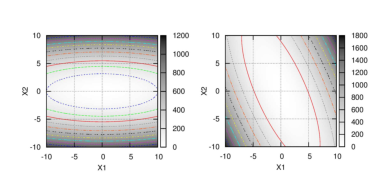
\includegraphics{ellipseB.eps}}
\end{minipage}
%\begin{minipage}[b]{0.5\linewidth}
% \centering
% \resizebox*{9cm}{!}{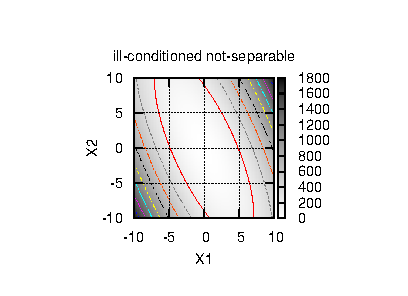
\includegraphics{ellipseturn.eps}}
%\end{minipage}
\caption{Separable (left) and non-separable (right) objective functions.} 
\label{nonsep}
\end{figure}

As mentioned above, an ill-posed optimization problem suffers from the curse of dimensionality, the computational cost to solve it scales superlinearly with the number of design variables N. To better understand this, let us first examine a separable objective function. The cost for solving an optimization problem with a separable objective function increases linearly with N, since the global optimum can be located by minimizing $N$ objective functions with a single design variable each (separately minimise $f_i(x_i),~ \forall x_i \in \vec{x}$). Thus, the cost of solving a separable $N$-dimensional optimization problem is approximately $N$ times the cost of solving the equivalent 1D problem. On the other hand, this is not possible for an ill-posed optimization problem since, for at least one design variable, its optimal value depends on the values some or all of the other take on. Since the search space increases exponentially with N, this leads to a superlinear (with N) increase in the cost of solving ill-posed problems.   
 
\subsection{Investigation of EAs Efficiency Degradation in Ill-Posed Problems}
\label{Inv2}

In order to investigate the effects of ill-posed optimization problems on EA's efficiency, two mathematical test cases with different N values are solved, both in their separable (well-posed) and non-separable (ill-posed) form. The results presented in this section correspond to the mean performance of $10$ runs, with different random number generator seeds. 

The first analytical test case to be examined is a multi-dimensional ellipsoid (a 2D version of it can be seen in fig.\ \ref{nonsep}) described, in its separable form, by   


\begin{eqnarray}
   f(\vec{x})=\sum^{N}_{i=1} a^{\frac{i-1}{N-1}}x_i^2
   \label{ellipse} 
\end{eqnarray}
where the value of $a$ determines the anisotropy of the objective function. Large values of $a$ lead to increasingly anisotropic functions.

The same problem can be examined after casting it in non-separable form, as follows

\begin{eqnarray}
   f(\vec{y})=\sum^{N}_{i=1}a^{\frac{i-1}{N-1}}y_i^2
   \label{ellipse} 
\end{eqnarray}
where $\vec{y}=B\vec{x}$ and $B$ is an appropriate $N\times N$ orthogonal rotation matrix.

In order to investigate both the effects of the design space dimension ($N$) and the condition number ($a$), four different optimization problems were solved. A 10D ($N\!=\!10$) optimization problem was solved for $a\!=\!10$ and $a\!=\!100$,  fig. \ref{ellipse_t1}, and a $N\!=\!30$ problem for $a\!=\!100$ and $a\!=\!1000$, fig. \ref{ellipse_t2}. 


\begin{figure}[h!]
\begin{minipage}[b]{0.5\linewidth}
 \centering
 \resizebox*{7.5cm}{!}{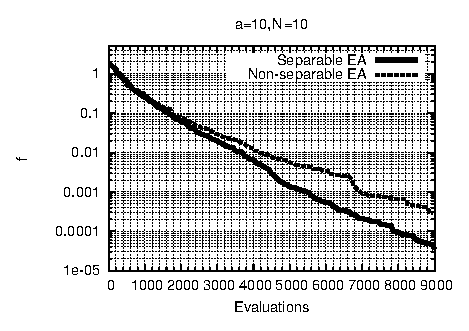
\includegraphics{10_10d.eps}}
\end{minipage}
\begin{minipage}[b]{0.5\linewidth}
 \centering
 \resizebox*{7.5cm}{!}{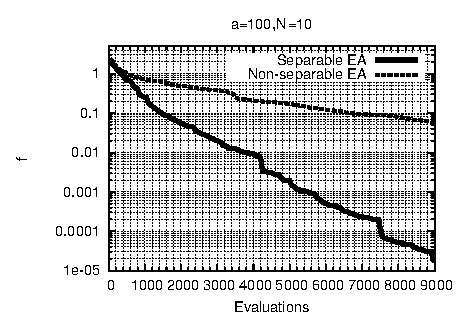
\includegraphics{100_10d.eps}}
\end{minipage}
\caption{10D ellipsoid. Condition number $a\!=\!10$ (left). Condition number $a\!=\!100$ (right). Increasing $a$ from $10$ to $100$  increases the EAs performance gap between the separable and non-separable problems.} 
\label{ellipse_t1}
\end{figure}

\begin{figure}[h!]
\begin{minipage}[b]{0.5\linewidth}
 \centering
 \resizebox*{7.5cm}{!}{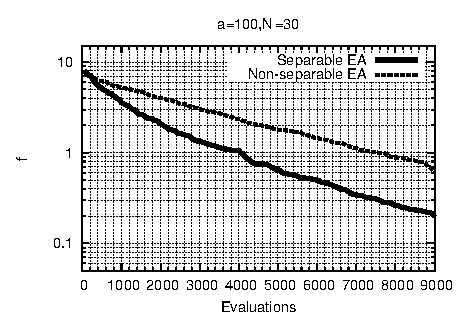
\includegraphics{100_30d.eps}}
\end{minipage}
\begin{minipage}[b]{0.5\linewidth}
 \centering
 \resizebox*{7.5cm}{!}{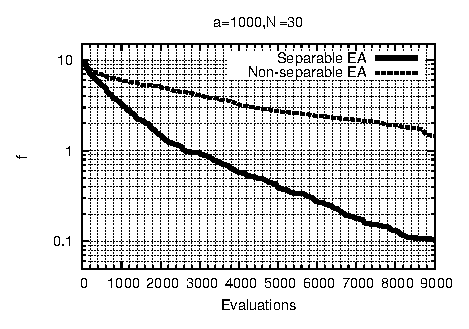
\includegraphics{1000_30d.eps}}
\end{minipage}
\caption{30D ellipsoid. Condition number $a\!=\!100$ (left).  Condition number $a\!=\!1000$ (right). As in the 10D case, increasing $a$ from $100$ to $1000$ causes additional losses in performance and increases the performance gap between separable and non-separable optimization problems.} 

\label{ellipse_t2}
\end{figure}

In figs. \ref{ellipse_t1} and \ref{ellipse_t2}, one may identify both the effects of increasing the condition number and increasing the problem dimension. A condition number with higher value leads to greater performance gap between the separable and non-separable cases, for both $N\!=\!10$ and $N\!=\!30$ cases. Increasing the problem dimension has the same effect. Focusing on the $a\!=\!100$ case, for both $N\!=\!10$ and $N\!=\!30$, one may observe that the difference in objective function values $|\Delta(f)|$, for the same computational cost of $9000$ evaluations, differ. For the $N\!=\!10$ case, $|\Delta(f)|\!=\!|f(non-separable)\!-\!f(separable)| \approx  10^{-4}$. On the other hand, for the $N=30$ case $|\Delta(f)| \approx  0.9$. This difference in $|\Delta(f)|$, between the 10D and 30D case, denotes a significant increase in the efficiency gap between separable and non-separable cases when the dimension is increased.      

The second analytical test case is concerned with the minimization of a multi-modal objective function described by  

\begin{eqnarray}
   f(\vec{x})=10N+(\sum^{N}_{i=1}x_i)^2 - 10N~ cos(\pi  \sum^{N}_{i=1}x_i)
   \label{mm} 
\end{eqnarray}

A 2D example is shown in fig.\ \ref{multimod}. As it appears in eq.\ \ref{mm}, the problem is non-separable. It can, though, easily be transformed to a separable one if $\vec{x}$ changes to $\vec{y}=B\vec{x}$, where $B$ is an appropriate rotation matrix.  A $45^o$ rotation is employed in each direction.  This objective function is extremely anisotropic since only one direction in the design space contributes to the objective function value and all the rest become irrelevant. Therefore, the condition number $a$ equals practically to $\infty$. This is an important class of objective functions since it resembles MOO problems as shown in section \ref{VCMM}.    

In order to investigate the effects of non-separability, as a function of the problems dimension, two optimization problems (5D and 30D) were solved.  
\begin{figure}[h!]
\begin{minipage}[b]{1\linewidth}
 \centering
 \resizebox*{14cm}{!}{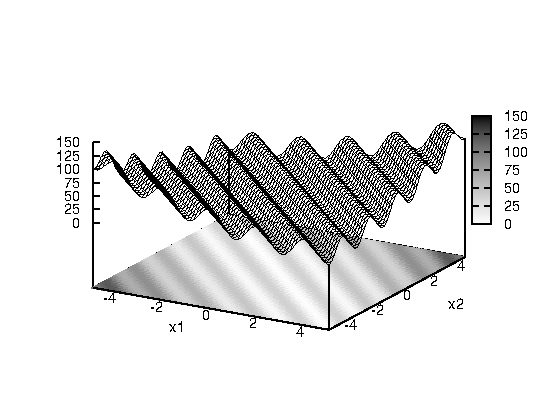
\includegraphics{multimodnomap.eps}}
\end{minipage}
%\begin{minipage}[b]{1\linewidth}
 %\centering
 %\resizebox*{11cm}{!}{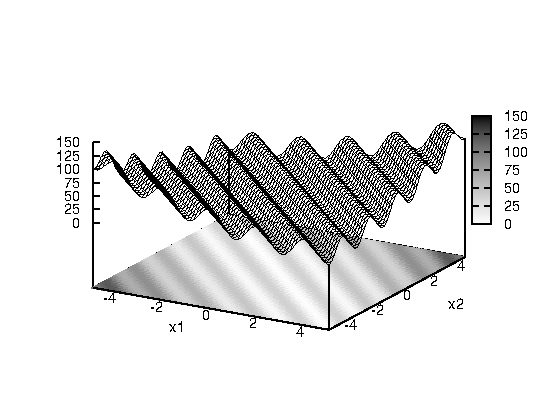
\includegraphics{multimodnomap.eps}}
%\end{minipage}
\caption{Minimization of eq. \ref{mm}, for N=2. The optimal value of $x_1$  depends on the choice of $x_2$ and vice-versa. So, this objective function is non-separable in terms of $x_1$ and $x_2$. Nevertheless, by aligning one of the two design variables with the $x_1\!=\!x_2$ axis, the problem becomes separable.} 

\label{multimod}
\end{figure}

In fig.\ \ref{multimodres}, it is demonstrated that both problems, if reformulated using  separable objective functions, outperform the non-separable ones. One may also observe that, the increase in problem's dimension causes an increase in efficiency gain, between separable and non-separable function cases. This conclusion is similar to the one made for the ellispoid test case. 



\begin{figure}[h!]
\begin{minipage}[b]{0.5\linewidth}
 \centering
 \resizebox*{7cm}{!}{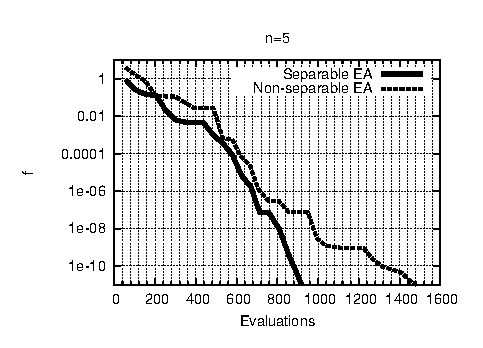
\includegraphics{5d.eps}}
\end{minipage}
\begin{minipage}[b]{0.5\linewidth}
 \centering
 \resizebox*{7cm}{!}{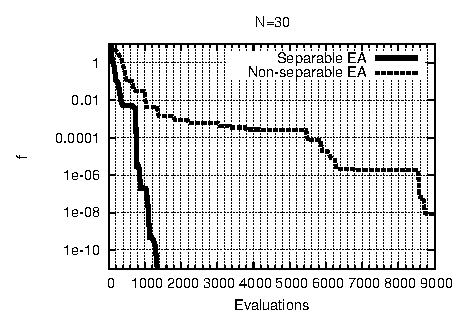
\includegraphics{30d.eps}}
\end{minipage}
\caption{Solution of the 5D problem of eq.\ref{mm} (left). Solution of the 30D problem of eq.\ \ref{mm} (right). The loss in efficiency for problems with extremely anisotropic objective functions increases significantly with the design space dimension.} 
\label{multimodres}
\end{figure}

Through the preformed investigations  (figs. \ref{ellipse_t1}, \ref{ellipse_t2} and \ref{multimodres}), it is convincingly shown  that a significant amount of the EA efficiency can be lost when dealing with ill-posed optimization problems, especially when these are combined with high values of N. The degree of efficiency deterioration is proportional to three quantities:

\begin{description}
  \item[a)] The anisotropy magnitude: Increasing anisotropy leads to less efficient EAs (figs.\ \ref{ellipse_t1} and \ref{ellipse_t2}).    
  \item[b)] Function separability: Problems with separable objective functions with respect to their design variables can be solved significantly faster using EAs, as shown in figs.\ \ref{ellipse_t1}, \ref{ellipse_t2} and \ref{multimodres}.  
  \item[c)] The number of design variables $N$: It is obvious that, by increasing the number of design variables, any EA requires more computational resources to locate the optimal solution. Additionally, if combined with (b), the great value of $N$ leads to superlinear increase in cost (fig. \ref{multimodres}).  
\end{description}

\section{Ill-Posed MOO Problems}
\label{VCMM}
In ill-posed MOO problems, all comments made and conclusions reached must now be applied to the scalar cost function $\Phi$ (rather than the objective function f), since $\Phi$ is the quantity which ``drives'' the evolution operators. In MOO, ill-posed optimization problem are typically associated with functions $\Phi$ which are non-separable and extremely anisotropic. This results from the fact that a Pareto front of optimal non-dominated solutions is sought. Since the $\Phi$ values given to the population members depend upon the Pareto dominance, all members of the current front of non-dominated solutions have $\Phi\!=\!0$ (or very small values compared to the dominated members of the population if niching effects are taken into account). These leads to directions in the design space that have very small impact on $\Phi$, i.e.\ directions along the Pareto front ($\Phi\!\approx\!0$) and directions with high impact on it, i.e those perpendicular to the Pareto front, therefore, almost always, resulting in an extremely anisotropic problem. 

\section{Principal Component Analysis}
The aim is to find the appropriate transformation of the original set of variables $\vec{x}  \rightarrow \vec{x}^*$, capable to transform the ill-posed optimization problem in hand into a better-posed one. After this transformation, the objective function in SOO or  the scalar cost function $\Phi$ in MOO is expected to have enhanced separability properties with respect to the transformed design variables $\vec{x}^*$.  This procedure is equivalent to finding an orthogonal matrix $U$ ($UU^T=I$) and based on it, express $\vec{x}^*$ as $\vec{x}^*=U\vec{x}$. In this thesis, it is proposed that the topological characteristics of the Pareto front determine the appropriate transformation matrix $U$.  To extract these in a way which best represents the data variance, the Principal Component Analysis (PCA) method is used, \cite{Hayk1999,Jolliffe_2002}. The transformation matrix $U$ contains the Principal Directions (PDs) computed by the PCA applied to the members of the Pareto front.   

However, the Pareto front is the final goal of the optimization process and therefore, it is unknown during the optimization.  Instead, in the proposed method, in each EA generation, the front of non-dominated solutions (elite set) is the one undergoing PCA. This is a reasonable choice since, as the evolution proceeds, the current elite-set tends to the Pareto front. Thus, the PDs computed by processing the elite-set in each generation become progressively more reliable approximations of the PDs computed by analysing the Pareto front.

Applying PCA to the current elite-set calls for the transformation of  its members into a standardized data-set $X$, with $\mu=0$ and $\sigma=1$ in all directions. Next step is the computation of the empirical covariance matrix $P$, \cite{Fodor_2002, Jolliffe_2002},

\begin{equation} 
   P= \frac{1}{e}XX^T
   \label{Cov_Mat} 
\end{equation}
where $e$ is the size of the elite-set and $X$ the matrix formed using  the members of the elite-set as columns. Then, via the spectral decomposition theorem, \cite{Axler_1997, Fodor_2002}, $P$ can be written as

\begin{equation} 
   P= U\Lambda U^T
   \label{spectral}
\end{equation}
where $\Lambda\!=\!diag(\lambda_1 , . . . , \lambda_N )$ is a diagonal matrix with the eigenvalues of $P$ and $U$ is a $N\!\times\!N$ matrix containing the eigenvectors (PDs) as columns. 

\FloatBarrier
\section{The Welded Beam Case}

To better demonstrate the ill-posed nature of MOO problems, a modified version of the welded beam case \cite{coello2000use} is used, (fig.\ \ref{case}).  The minimization of both the cost ($K$) and the deflection ($\Delta$) of a welded beam subject to force $P$ (fig.\ \ref{case}) is desired. There are two design variables: the welding length ($x_1$ or $l$)  and the side length of the square cross section ($x_2$ or $t$). The design is subject to three constraints regarding shear stress ($\tau$), bending stress ($\sigma$) and buckling load ($P_c$).    


%\figuremacroW{case}{Welded beam case - Problem definition.}{In the examined case, design variables are square cross section side-length ($X_2 = t$) and welding length ($X_1 = l$) are the design variables.}{0.4}

The problem requires the minimization of both the cost
%\begin{equation} 
\begin{eqnarray}\nonumber
   K = 1.10471h^2l+0.04811t^2(14.0+l) %\\
%   = 1.10471h^2X_1+0.04811X_2^2(14.0+X_1)
   \label{Cost} 
\end{eqnarray}
and the deflection
%\end{equation}
\begin{eqnarray}
   \Delta = \frac{4PL^3}{Et^4} = \frac{4PL^3}{EX_2^4}
   \label{Deflection} 
\end{eqnarray}

\begin{figure}
\begin{minipage}[b]{1\linewidth}
 \centering
 \resizebox*{5cm}{!}{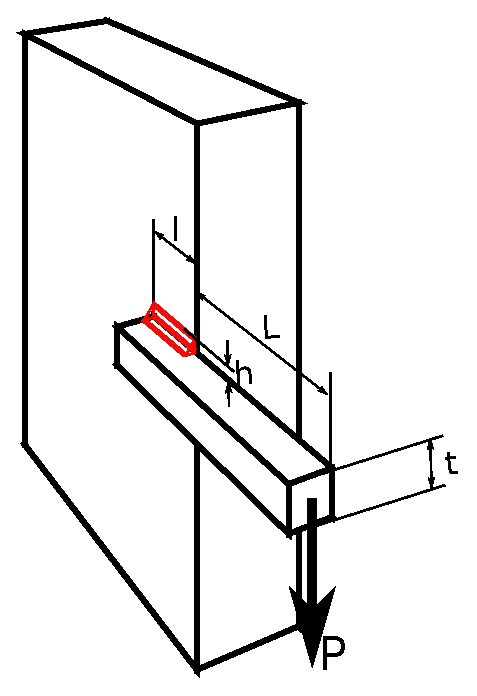
\includegraphics{case.eps}}
\end{minipage}
\caption{The Welded Beam Case: In the examined case, the welding length ($x_1\!=\!l$) and the square cross section side-length ($x_2\!=\!t$)  are the two design variables.} 
\label{case}
\end{figure}



The first constraint is related to the shear stress applied to the welding in order to ensure its structural integrity. The maximum shear stress depends on the type and quality of the welding.  This constraint is expressed as 
\begin{eqnarray}
   \tau = \sqrt{\tau_1^2 + \frac{\tau_1 \tau_2 l}{R} +\tau_2^2} \leq 13600 psi
\label{shear}
\end{eqnarray}
where
\begin{eqnarray}
   \nonumber \tau_1 = \frac{P}{\sqrt{2}hl}, ~~~\tau_2 = \frac{MR}{J}, ~~~M = P(L+\frac{l}{2}) 
\end{eqnarray}
\begin{eqnarray}
   \nonumber R = \sqrt{\frac{l^2}{4} + (\frac{h+t}{2})^2} 
\end{eqnarray}
\begin{eqnarray}
   \nonumber J = 2\left( \sqrt{2}hl\left( \frac{l^2}{12} + \left(\frac{h+t}{2}\right)^2 \right) \right)
\end{eqnarray}

The second constraint is on the bending stress applied to the beam, in order to ensure its structural integrity. The maximum bending stress depends on the beam material,
\begin{eqnarray}
   \sigma = \frac{6PL}{t^3} \leq 30000 psi
   \label{bend} 
\end{eqnarray}

Finally, in order to avoid buckling, the buckling load is also constrained as follows,  
\begin{eqnarray}
   P_c = \frac{4.013E\sqrt{\frac{t^8}{36}}}{L^2}\left( 1- \frac{t}{2L}\sqrt{\frac{E}{4G}} \right) \geq P 
   \label{back} 
\end{eqnarray}
where the welding height is $h \! = \!0.6 in$, the beam length is $L \! =\! 14 in$, the force is $P\! =\! 6000 lb$, the Young’s modulus is $E \!=\! 30 \! \times \! 10^6 psi$ and the shear modulus is $G\! = \!12 \! \times \! 10^6 psi$.  

Apart from the constraints which are related to structural integrity, two additional constraints, related to both objectives, were imposed. These are 
\begin{eqnarray}
   K \leq 50 \\
   \Delta \leq 0.25 
   \label{obj} 
\end{eqnarray}


%\begin{figure}[h!]
%\begin{minipage}[b]{0.5\linewidth}
% \centering
% \resizebox*{7cm}{!}{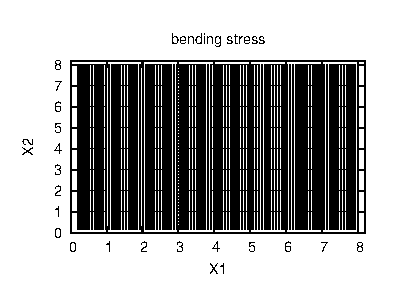
\includegraphics{Const_sx.eps}}
%\end{minipage}
%\begin{minipage}[b]{0.5\linewidth}
% \centering
% \resizebox*{7.5cm}{!}{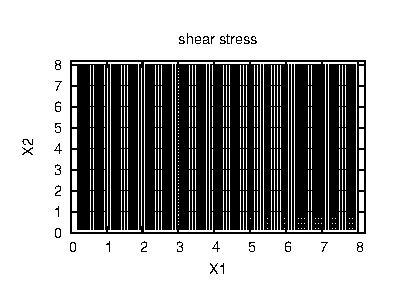
\includegraphics{Const_tx.eps}}
%\end{minipage}
%\begin{minipage}[b]{0.5\linewidth}
% \centering
% \resizebox*{7.5cm}{!}{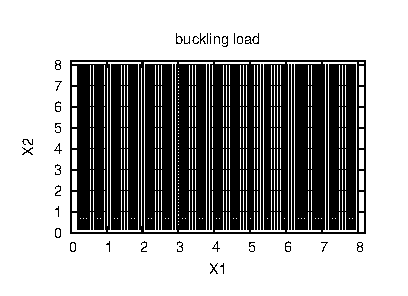
\includegraphics{Const_P.eps}}
%\end{minipage}
%\begin{minipage}[b]{0.5\linewidth}
% \centering
% \resizebox*{7.5cm}{!}{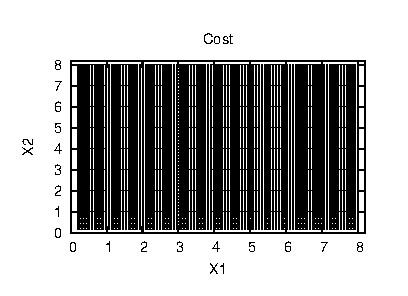
\includegraphics{Const_Price.eps}}
%\end{minipage}
%\begin{minipage}[b]{0.5\linewidth}
% \centering
% \resizebox*{7.5cm}{!}{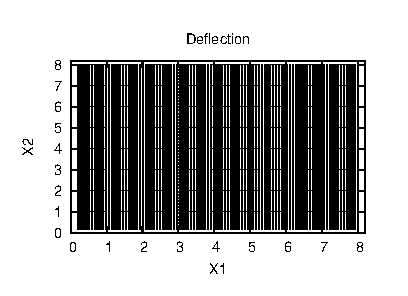
\includegraphics{Const_Dx.eps}}
%\end{minipage}
%\begin{minipage}[b]{1\linewidth}
% \centering
% \resizebox*{12cm}{!}{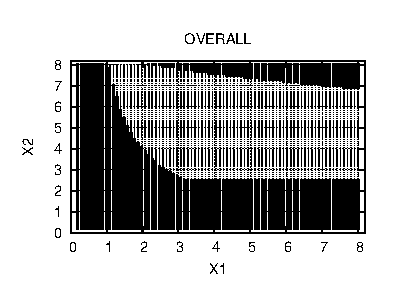
\includegraphics{Const_ALL.eps}}
%\end{minipage}

%\caption{Investigation of the feasibility of the design $(X_1,X_2)$ plane. The overall feasible design space is presented in the lower right figure with white squares.} 
%\label{x1x2}
%\end{figure}

%This case was deliberately chosen as a demonstration case due to the clear physical meaning of the relations that appear between its design variables. By carefully examining the objectives it is clear that in order to decrease deflection $X_1$ must be increased(eq. \ref{Deflection}). However any increase in $X_1$ will lead to higher cost (eq. \ref{Cost} ). In order to keep cost stable $X_2$ must simultaneously decrease, this of-course is bounded by the structural constraints (eq. \ref{shear},\ref{bend} and \ref{back}). 
 
From the  $\Phi$ plot shown in fig.\ \ref{reco1} (left), it is evident that the problem in hand is both extremely anisotropic and non-separable (ill-posed). Using the proposed PCA of the elite-set (fig.\ \ref{reco1}, right) the computed PDs point to the directions in the design space which if used to define new design variables, would transform the ill-posed problem into a better-posed one. The direction with the largest eigenvalue $\lambda_1$ is the direction that describes the Pareto front is aligned with the $\Phi=0$ curve. On the other hand, the PD with the smallest eigenvalue $\lambda_2$ is the direction in the design space which corresponds to the largest change in $\Phi$ values. Smaller eigenvalue means smaller variance in the corresponding direction, in the elite-set. % Thus the EA, through its evolution operators, restricted the values of this direction within a small band of values denoting its importance regarding $\Phi$. 

%Looking at the physical meaning of the correlations between the design variables in the welded beam case; $e_1$ suggest that if one desires to move along the  $\Phi=0$ front he should either increase $X1$ (welding length) and decrease $X2$ (cross section) or vise vesra. In other words one can move from, say, expensive designs with small deflection to cheap designs with bigger deflection (fig.\ref{Pareto1}) by reducing the cross section but in order to keep respecting the various stress constraints (fig.\ref{x1x2}) one should simultaneously increase the welding length. On the other hand $e_2$ suggest that if one wants to move on the direction that would cause the biggest difference in $\Phi$ he should either increase or decrease both $X1$ \& $X2$ simultaneously.          

\begin{figure}[h!]
\begin{minipage}[b]{1\linewidth}
 \centering
 \resizebox*{!}{4.5 cm}{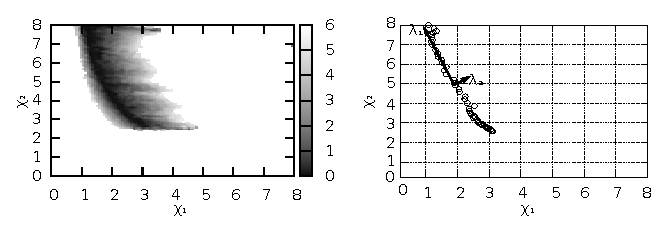
\includegraphics{DOFs.eps}}
\end{minipage}
%\begin{minipage}[b]{0.5\linewidth}
% \centering
%\resizebox*{8cm}{!}{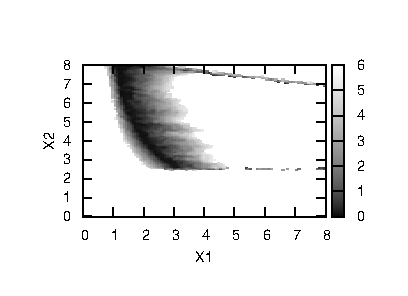
\includegraphics{CaseCorr.eps}}
%\end{minipage}
\caption{The Welded Beam Case: Left; $\Phi$ iso-areas over the design space, at a specific generation during the evolution. Right; The elite-set, plotted in the design space. Based on it, two PDs denoted by $\lambda_1$ and $\lambda_2$ are computed.} 
\label{reco1}
\end{figure}

\begin{figure}[h!]
\begin{minipage}[b]{1\linewidth}
 \centering
 \resizebox*{!}{7 cm}{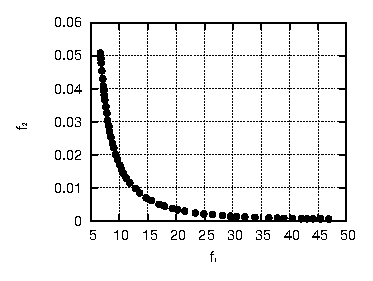
\includegraphics{Pareto.eps}}
\end{minipage}
\caption{The Welded Beam Case: The elite-set shown in fig.\ref{reco1} is plotted in the objective space, where $f_1$ = cost and $f_2$ = deflection.} 
\label{Pareto1}
\end{figure}


\section{PCA-Driven Evolution Operators} 
%The PCA driven evolution operators to better ``drive'' evolution by utilising the information about the design variable correlations are proposed here as a method to deal with ill-posed optimization problems. To be more specific, PCA is used to identify the relations in the form of direction in the design space. The design space is, then, temporarily aligned with these directions, the necessary evolution operators apply to the so--rotated space and, finally, the generated offspring are transformed back to the original design space. Any sort of dimensionality reduction or rotation of the design space occurs just before (and after) the application of the evolution operators. To initiate PCA, a small number of representative solutions to the problem must be available; this set is dynamically updated during the evolution. In MOO applications, this comprises the members of the current front of non--dominated solutions. In SOO problems, in which there is no set of non--dominated solutions, the principal components can be found by processing a user--defined number of top individuals in the current offspring population. It is evident that, as the evolution proceeds, and the current front of non--dominated solutions converges to the Pareto front, the principal components approach those of the Pareto front. 
In EA-based optimization, the application of the evolution operators may benefit a lot from the outcome of PCA, in order to reduce the computational cost required for the same quality of solutions. To be more specific, PCA is used to identify directions in the design space which, if used to define new optimization variables, would lead to an optimization problem with (almost) separable objective function. The design space is, then, temporarily aligned with the principal directions and the evolution operators apply to individuals expressed in the so-rotated axes. At the end of this phase, the generated offspring are transformed back to the original axes of the design space. The rotation of the design space axes occurs just before and after the application of the evolution operators thus deeming it transparent to the designer. To perform the PCA, a small number of well-performing solutions to the problem must be available. Herein, these are the members of the current elite-set, as stated before; this set is dynamically updated during the evolution. In MOO applications, the elite-set comprises the members of the current front of non--dominated solutions. In SOO problems, where the notion of dominality degenerates, the PDs  can be found by processing a user--defined number of the current top individuals. 

Let the aligned with the PDs design vectors \(\vec{x}_i\) be represented by \(\vec{x}^*_i\). The alignment is performed as follows
\begin{equation} 
   \vec{x}^*_i=U(\vec{x}_i-\vec{\mu}_{X})
   \label{align} %http://users.ics.tkk.fi/jhollmen/dippa/node30.html
\end{equation}
where $\vec{\mu}_{X}$ is the vector of mean (over the elite set) design variables.
The inverse transformation, from $\vec{x}^*_i$ to $\vec{x}_i$, is given by
\begin{equation} 
   \vec{x}_i=U^{-1}\vec{x}^*_i+\vec{\mu}_{X}
	\label{re-align}
\end{equation}
It should be stated that the CPU cost to compute \(U^{-1}\) is negligible since U is an orthogonal matrix and, thus, \(U^{-1} = U^T\). 

The two main PCA-driven evolution operators, recombination and mutation, are presented below.  

\paragraph{}
\subsection{PCA-Driven Recombination}
The recombination operator is applied to the rotated design variable-set which are sought to be as separable as possible. As shown in fig.\ \ref{reco2}, this changes the probability of the offspring appearance in the design space as if the problem was separable (fig.\ \ref{reco1}). 

\begin{figure}[h!]
\begin{minipage}[b]{0.5\linewidth}
 \centering
 \resizebox*{7cm}{!}{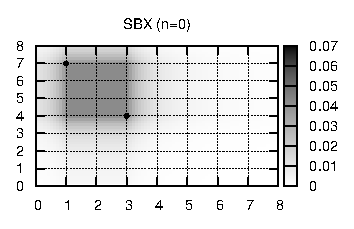
\includegraphics{SBX3dparents2a.eps}}
\end{minipage}
\begin{minipage}[b]{0.5\linewidth}
 \centering
 \resizebox*{7cm}{!}{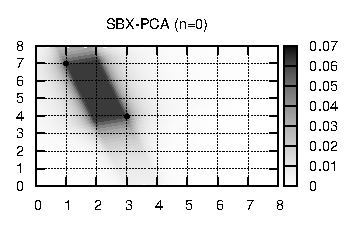
\includegraphics{SBX3dparentsPCAa.eps}}
\end{minipage}
\caption{The Welded Beam Case: The  Offspring appearance probability using the SBX(n=0) recombination scheme (section \ref{RecombinationLabel}). Assume that there are two  parents shown by the two black dots. Left; SBX recombination. Right; PCA driven SBX recombination.} 
\label{reco2}
\end{figure}

From figs.\ \ref{reco1} and \ref{reco2}, it can be seen that the proposed method assigns higher offspring appearance probability to the regions near $\Phi\!=\!0$ which is the region that accommodates the currently best (elite) individuals. Therefore, the PCA-driven recombination  better achieves its goal of mixing, according to the building block hypothesis \cite{Gold89}. Mixing is the process in which building blocks (low-order schemata of high fitness) are combined to form new potentially fit schemata of higher order. The proposed method increases the probability individuals generated through the application of the recombination operator to be fit.   

%\begin{figure}[h!]
%\begin{minipage}[b]{1\linewidth}
% \centering
% \resizebox*{10cm}{!}{\includegraphics{ellipseturn_eig.eps}}
%\end{minipage}
%\caption{Example $\Phi'$ plot for} 
%\label{phi1}
%\end{figure}


\subsection{PCA-Driven Mutation}
Mutation is also applied to the design space aligned with the computed PDs. The mutation probability on each PD is dynamically updated based on the variance ($\vec{V}$) of the elite population members, projected onto the aforementioned direction ($V(i)$), eq. \ref{alignMut}. This is done in a way that keeps the overall mutation probability per individual constant (and equal to a user-defined value). The proposed method distributes the mutation probability among the PDs  in a way which is proportional to the importance of each direction, according to the characteristics of the current front of non-dominated solutions. As shown in the welded beam case, the importance of each PD, regarding either f (SOO) or $\Phi$ (MOO), is inversely proportional to its eigenvalue which quantifies the variance.  PDs  with high-valued eigenvalues receive smaller mutation probability, in contrast to the directions with low-valued eigenvalues which undergo mutation with higher probability. The formula used to adjust the mutation probability (per each newly computed direction (index $i$)) is        

\begin{equation}
	p_m^i = 0.1 p_m + \frac{0.9 p_m N}{D_V} \cdot \frac{V_{max}-V_i}{V_{max}-V_{min}} 
     \label{alignMut}
\end{equation}
where $p_m$ is a user--defined mutation probability,  
$V_{max}=\mbox{max}\{V_1,...,V_N\}$, $V_{min}=\mbox{min}\{V_1,...,V_N\}$ and 
\begin{equation}
	D_V=\sum_{i=1}^N \frac{V_{max}-V_i}{V_{max}-V_{min}}
\label{alignMut2} %http://users.ics.tkk.fi/jhollmen/dippa/node30.html
\end{equation}


%\begin{equation} 
%   P_m^{i}=0.1 P_m + \frac{0.9 P_m N}{P_m^{gl}} (1-\frac{(V_i-min(\vec{V}))}{(max(\vec{V})-min(\vec{V}))}),~~~~i=1,N 
%   \label{alignMut} %http://users.ics.tkk.fi/jhollmen/dippa/node30.html
%\end{equation}
%where $P_m$ is the user-defined mutation probability, N the number of design variables and 
%\begin{equation} 
%   P_m^{gl}=\sum^{N}_{i=1} 1-\frac{(V_i-min(\vec{V}))}{(max(\vec{V})-min(\vec{V}))}
%   \label{alignMut2} %http://users.ics.tkk.fi/jhollmen/dippa/node30.html
%\end{equation}



Let us denote  by $g$ the generation counter, by $k_{DB}$ the number of currently existing entries into the DB and by $k_{min}$ the minimum number of entries needed to initiate the use of the metamodel--based pre--evaluation phase. Then, the successive steps of the PCA--driven MAEA or MAEA(PCA) can be described as follows:
\begin{description}
  \item[Step 1:] For the current offspring population $S^{g}_\lambda$, set $\lambda^*\!=\!\lambda$ (if $k_{DB}\!<\!k_{min}$) or  $\lambda^*\!=\!\lambda_{e}$ (else), where $\lambda_{e}$ the number of offspring to be evaluated on the problem--specific evaluation software. 
  \item[Step 2:] If $k_{DB}\!\ge\!k_{min}$, $\lambda$ RBF networks are trained on paired input--output patterns selected from the DB, in the vicinity of each offspring. Pre--evaluate the $\lambda$ population members on the so--trained metamodels. Select the $\lambda_{ex}$ top of them, based on dominance and proximity criteria.
  \item[Step 3:] Evaluate the $\lambda_{e}$ offspring on the problem--specific evaluation software. Update $S^{g}_e$.
  \item[Step 4:] Compute the current set of PDs  based on the updated elite-set $S^{g}_e$ (eqs. \ref{Cov_Mat} and \ref{spectral}).
  \item[Step 5:] Align the design space with the so--computed PDs  (eq. \ref{align}). 
  \item[Step 6:] Create the new offspring population $S^{g+1}_\lambda$ through the application of the evolution operators to the aligned individuals. Re--align the generated offspring with the original design space coordinate system (eq.~\ref{re-align}).
  \item[Step 7:] Set $g\!\leftarrow\!g\!+\!1$; go to Step 1.
\end{description}
The above algorithm can readily be transformed to EA(PCA) by eliminating the use of metamodels or by setting $k_{min}$ to an ``infinite'' number.  
%\figuremacroW{MAEAPCA2}{MAEA-PCA}{Schematic representation of the PCA-driven MAEA algorithm.}{1.0}
%\begin{figure}[h!]
%\begin{minipage}[b]{1\linewidth}
% \centering
% \resizebox*{14cm}{!}{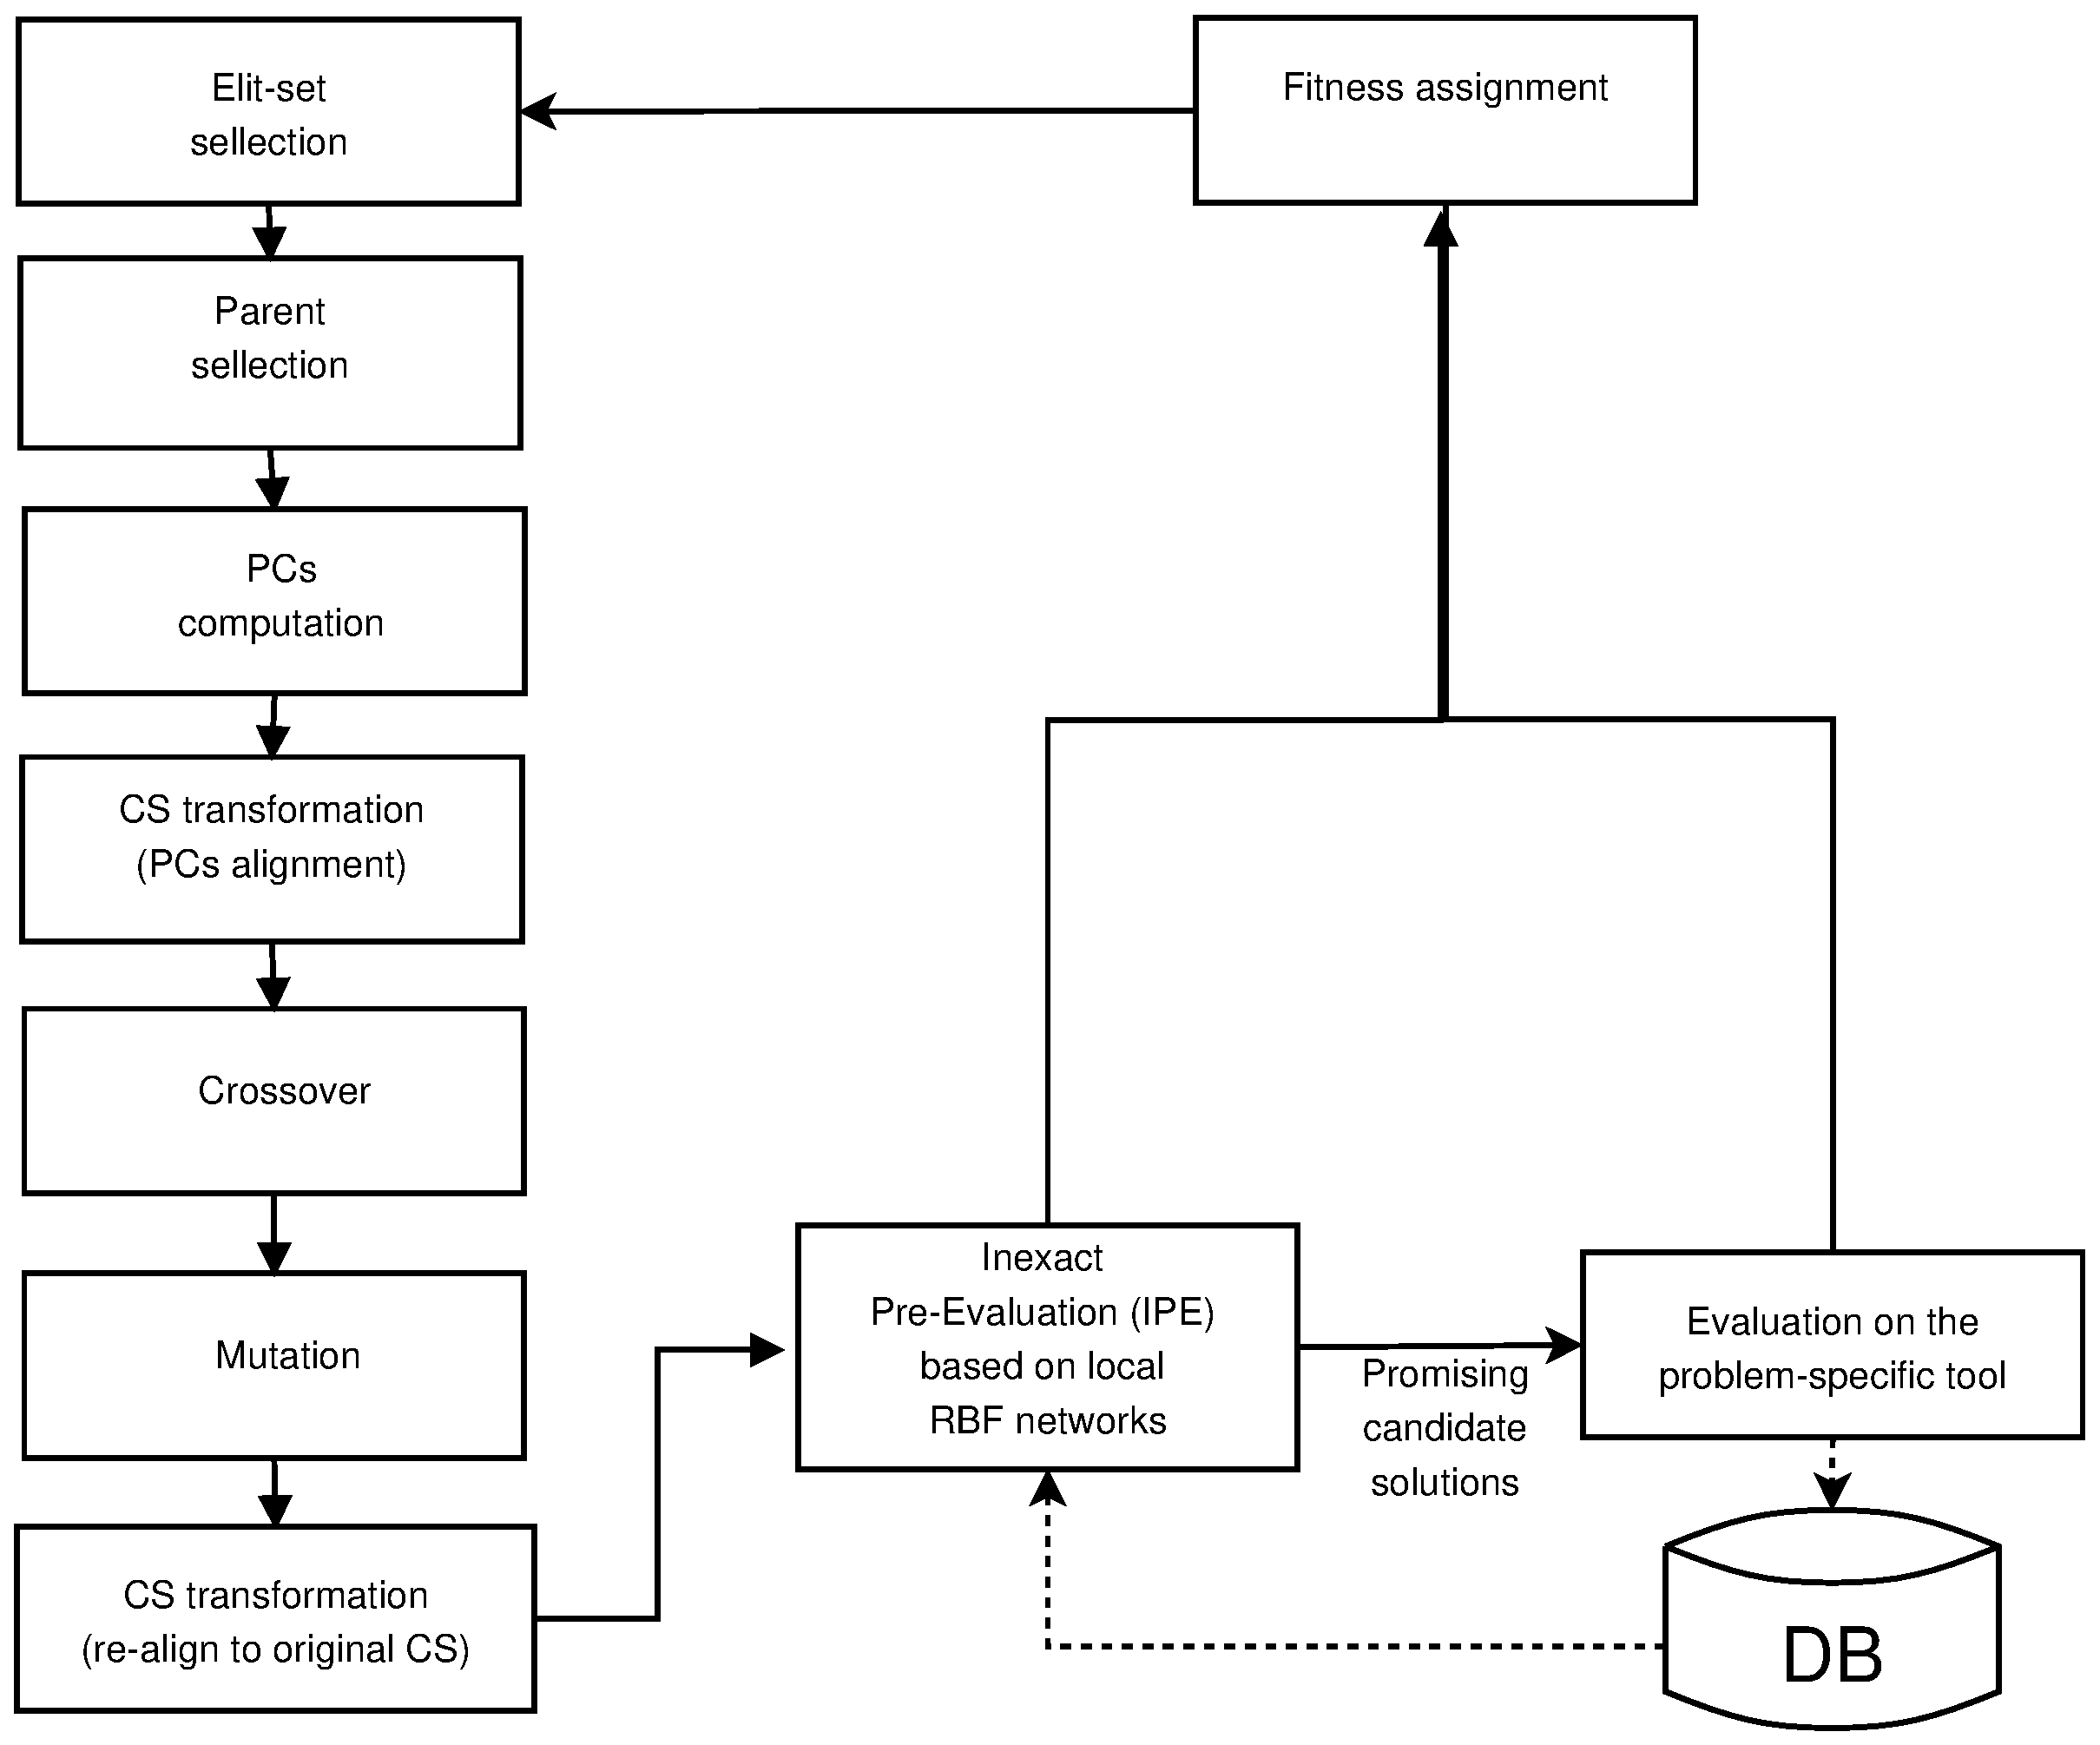
\includegraphics{MAEAPCA2.eps}}
%\end{minipage}
%\caption{Schematic representation of the PCA-driven MAEA algorithm.} 
%\label{MAEAPCA2}
%\end{figure}


%\figuremacroW{HypervolumeComparison}{Hypervolume Comparison}{Hypervolume comparison between EA and EA(PCA), metamodels where not used due to the fast evaluation time of The The The The The The The The The The Welded Beam Case: EA(PCA) outperforms traditional EA even though the dimensionality of the problem in hand is very low.}{0.9}

\subsection{Gain from the Use of EA(PCA)}

In order to demonstrate the performance gain from the use of the EA(PCA), the welded beam case and the two mathematical minimization problems already presented in section \ref{Inv2} are revisited. For each one of them, 10 runs were performed with different random number generator seeding. 

Regarding the two-objective welded beam problem, the average hypervolume indicator plotted in terms of the number of evaluations performed is presented in fig. \ref{HypervolumeComparison}. In this figure, it is shown that, even though the dimension of the problem was deliberately kept low ($N\!=\!2$) to facilitate the visual analysis of the obtained results, the gain from the use of the proposed method over the conventional EA is clear.  

\begin{figure}[h!]
\begin{minipage}[b]{1\linewidth}
 \centering
 \resizebox*{10cm}{!}{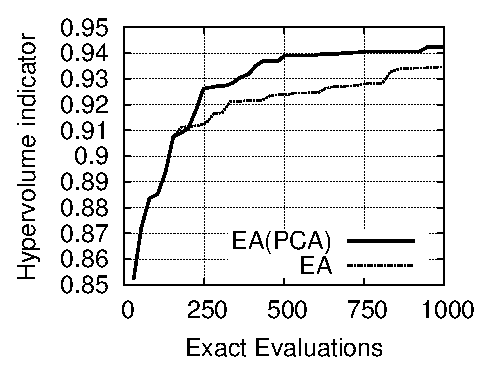
\includegraphics{HypervolumeComparison.eps}}
\end{minipage}
\caption{The Welded Beam Case: Average evolution of the hypervolume indicator using EA and EA(PCA). In this case, metamodels are not used due to the extremely small computational cost of each evaluation run. EA(PCA) outperforms traditional EA even though the dimensionality of the problem is very low.} 
\label{HypervolumeComparison}
\end{figure}



The comparison between conventional evolution operators and the PCA-driven ones, on the 30D non-separable ellipsoid with $a\!=\!1000$ (eq. \ref{ellipse}), is presented in fig.\ \ref{Ellt3}. This figure presents the mean objective function values of $10$ runs. 

\begin{figure}[h!]
\begin{minipage}[b]{1\linewidth}
 \centering
 \resizebox*{10cm}{!}{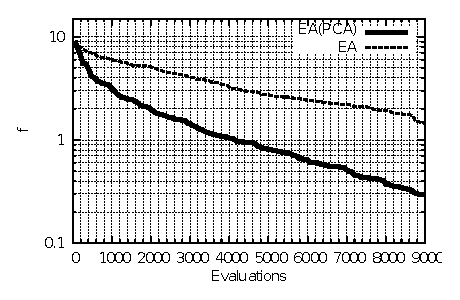
\includegraphics{1000_30d_pca.eps}}
\end{minipage}
\caption{30D non-separable ellipsoid with a=1000: Average convergence using EA and EA(PCA). The proposed PCA-driven evolution operators significantly outperform the conventional ones.} 
\label{Ellt3}
\end{figure}

In fig.\ \ref{Ellt3}, the significant gain from the use of the proposed EA(PCA) in comparison with an EA in the 30D ellipsoid case is shown.

Regarding the multi-dimensional and multi-modal problem of eq.\ \ref{mm} with N=30, a comparison between PCA-driven and conventional evolution operators is presented in fig.\ \ref{mmt3}.  In this figure, it is shown that the use of PCA-driven evolution operators significantly enhances the EA efficiency in the 30D multi-modal problem, too.


\begin{figure}[h!]
\begin{minipage}[b]{1\linewidth}
 \centering
 \resizebox*{10cm}{!}{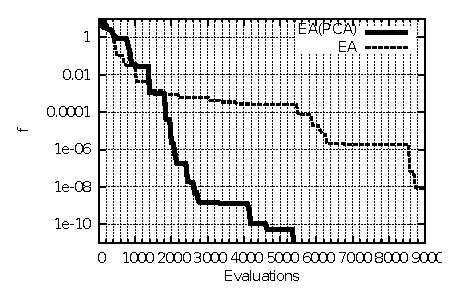
\includegraphics{30d_pca.eps}}
\end{minipage}
\caption{30D multi-modal problem: Average convergence using the EA and the EA(PCA). Similar to fig.\ \ref{Ellt3}, the proposed PCA-driven evolution operators significantly outperform the traditional ones.} 
\label{mmt3}
\end{figure}


%\FloatBarrier
\section{EAs Assisted by PCA-Driven Metamodels}
In MAEAs, the main challenge regarding the use of artificial neural networks as metamodels is to overcome the so--called curse of dimensionality in problems with a large number of design variables. 
The number of training patterns required to build a reliable metamodel increases with N; a side--effect is that their training becomes computationally costly. On the other hand, the need for more training patterns per metamodel delays the commencement of the IPE phase during the MAEA, until the DB collects a substantial number of entries. This leads to a further increase in the wall clock time of the optimization run.

This thesis proposes the reduction in the number of the RBF network sensory (input) nodes and, consequently, the required number of training patterns. The eigenvectors computed through the PCA of the elite-set are associated with the objective function variance. 
If the elite-set is expressed in a coordinate system aligned with the PDs, it is expected that any plot of the objective function (SOO) or $\Phi$ (MOO) in terms of the first components (i.e. those with the highest variance) must be scattered enough. In contrast, along the PDs with small variances, the elite members are much less scattered. 

The proposed method takes advantage of the above and cuts off a pre-selected number of the RBF network sensory units, particularly those related to the highest variance directions in the design space. As a result, the RBF networks are trained on lower dimension data. 
This truncation is applied only during the RBF network training, by firstly rotating/aligning all the selected training patterns with the computed PDs and, then, cutting those sensory nodes which correspond to the highest eigenvalues off. The number of the components to be cut off is user-defined.
    
% The use of the IPE technique, in its standard form, would require the use of RBF networks with two sensory nodes each, trained on neighbouring to the candidate solution, already evaluated stored individuals as shown in figure \ref{2dann}. 
    
    
%\begin{figure}[h!]
%\begin{minipage}[b]{1\linewidth}
% \centering
% \resizebox*{15cm}{!}{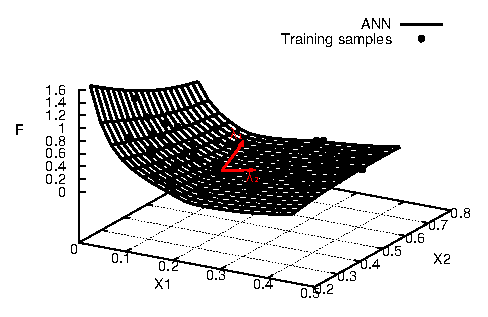
\includegraphics{2dANN.eps}}
%\end{minipage}
%\caption{Welded beam test problem: ANN with two sensory node used as metamodel in the standard IPE form. The ANN prediction is plotted as a surface grid and the training patterns used for its training as dots.} 
%\label{2dann}
%\end{figure}

\begin{figure}
\begin{minipage}{0.48\textwidth}
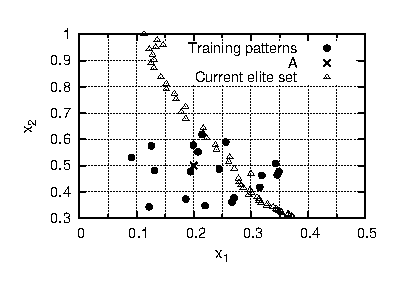
\includegraphics[scale=1.2]{IPE/x1_x2.eps}
\end{minipage}
\begin{minipage}{0.48\textwidth}
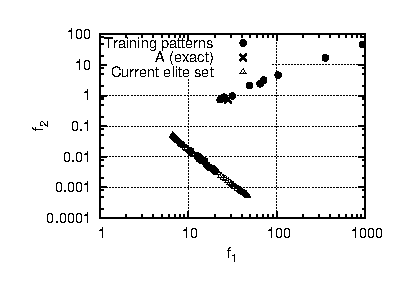
\includegraphics[scale=1.2]{IPE/f1_f2.eps}
\end{minipage}
\caption{The Welded Beam Case: An instant of the evolution process, where the current elite set, a candidate solution (A) and the training patterns selected from the current DB for training the metamodel to be used to predict the objective function value at A are plotted in the design (left) and objective (right) space.}
\label{fig:f1f2}
\end{figure}

Fig.\ \ref{fig:f1f2} presents an instant of the evolution process, at the end of the $6^{\mbox{th}}$ generation of one of the runs. At this instant, $\lambda$ new offspring have just been generated. Let us assume that the candidate solution A, with $(x_1, x_2)\!=\!(0.2,0.5)$  shown in fig.\ \ref{fig:f1f2}, needs to be pre-evaluated using an appropriately trained local RBF network. 
For this purpose, $19$ patterns are selected from the DB using the standard selection procedure. 
In fig.\ \ref{fig:f1f2}, the training patterns, the candidate solution and, also, the current elite-set are plotted both in the design ($x_1, x_2$) and objective ($f_1, f_2$) spaces. 
The exact values of $f_1$ and $f_2$ for A are also shown.
It is evident that, in a problem with only two design variables, there is no reason to reduce the number of design variables during the training of the RBF networks. However, it was decided to do so, just for the purpose of demonstration.  

\begin{figure}
\begin{minipage}{0.48\textwidth}
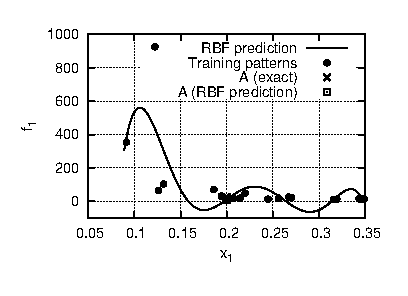
\includegraphics[scale=1.2]{IPE/f1_x1.eps}
\end{minipage}
\begin{minipage}{0.48\textwidth}
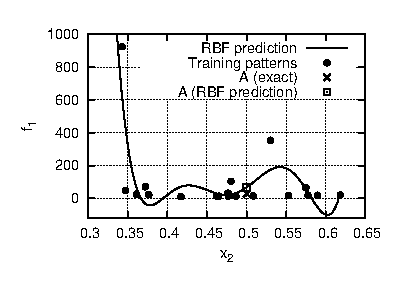
\includegraphics[scale=1.2]{IPE/f1_x2.eps}
\end{minipage}
\caption{The Welded Beam Case: RBF network predictions of $f_1$ if $x_1$ (left) and $x_2$ (right) are separately applied to the single sensory unit of the network. }
\label{fig:f1x1x2}
\end{figure}

\begin{figure}
\begin{minipage}{0.48\textwidth}
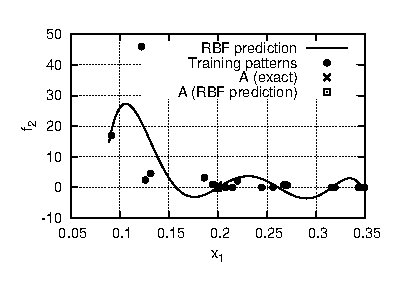
\includegraphics[scale=1.2]{IPE/f2_x1.eps}
\end{minipage}
\begin{minipage}{0.48\textwidth}
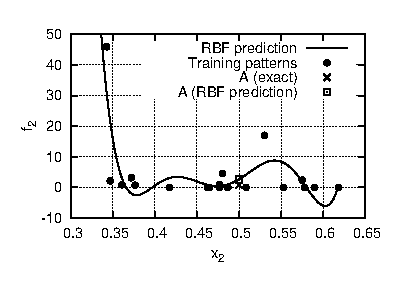
\includegraphics[scale=1.2]{IPE/f2_x2.eps}
\end{minipage}
\caption{The Welded Beam Case: RBF network predictions of $f_2$ if $x_1$ (left) and $x_2$ (right) are separately applied to the single sensory unit of the network. }
\label{fig:f2x1x2}
\end{figure}

A first demonstration of the proposed method is based on the welded
beam problem (fig.\ \ref{case}). In fig.\ \ref{fig:f1x1x2}, the $f_1$ predictions using two RBF networks, with either $x_1$ or $x_2$ as the only sensory unit of each network, are shown. Though these networks, after being trained on the selected $19$ patterns, must be used to predict the objective functions only at A, it is interesting to observe the overall deviation between the continuous line which stands for the network response and the training patterns' responses. 
Recall that the number of RBF centers is less than the number of training parameters, so the network does not interpolate the training patterns.
The observed high deviations, which could be even higher for some other candidate solutions, are easily explained by the fact that a two-variable function $f_1(x_1,x_2)$ is handled as $f_1(x_1)$ or $f_1(x_2)$. The corresponding results for $f_2$, instead of $f_1$, are shown in fig.\ \ref{fig:f2x1x2}. 
The exact objective function values at A along with the RBF predictions are tabulated in table \ref{tab:f1f2x1x2}. It can be seen that $f_1$ is predicted with a relative error of  $\approx \! 57\%$ if $f_1\!=\!f_1(x_1)$ and $\approx \! 138\%$ if $f_1\!=\!f_1(x_2)$ and the error of $f_2$ is  $\approx \! 110\%$ if $ f_2\!=\!f_2(x_1)$ and $\approx \! 260\%$ if $ f_2\!=\!f_2(x_2)$.


\begin{figure}
\begin{minipage}{0.48\textwidth}
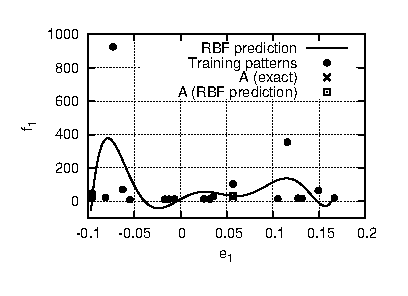
\includegraphics[scale=1.2]{IPE/f1_e1.eps}
\end{minipage}
\begin{minipage}{0.48\textwidth}
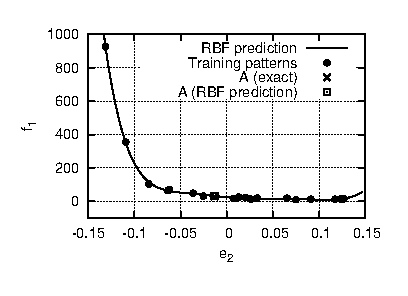
\includegraphics[scale=1.2]{IPE/f1_e2.eps}
\end{minipage}
\caption{The Welded Beam Case: RBF network predictions of $f_1$ if $e_1$ (left) and $e_2$ (right) are separately applied to the single sensory unit of the network.}
\label{fig:f1e1e2}
\end{figure}

\begin{figure}
\begin{minipage}{0.48\textwidth}
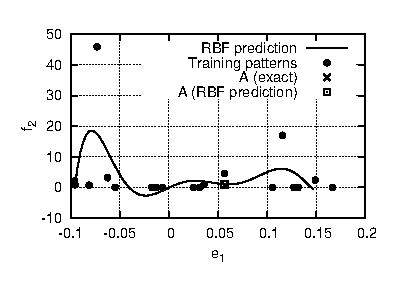
\includegraphics[scale=1.2]{IPE/f2_e1.eps}
\end{minipage}
\begin{minipage}{0.48\textwidth}
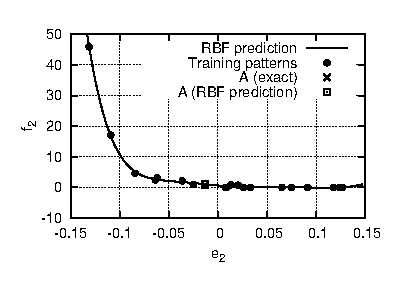
\includegraphics[scale=1.2]{IPE/f2_e2.eps}
\end{minipage}
\caption{The Welded Beam Case: RBF network predictions of $f_2$ if $e_1$ (left) and $e_2$ (right) are separately applied to the single sensory unit of the network. }
\label{fig:f2e1e2}
\end{figure}

\begin{table}[h!]
\begin{center}
\begin{tabular}{c  c | c | c}
		&      Exact  	 		&  RBF network predictions    &  RBF network  predictions   \\
		&  $(f_1,f_2)$ values   &  assuming $f_i=f_i(x_1)$    &   assuming $f_i=f_i(x_2)$  \\
		\hline
$f_1$	& $28.07$   &      $11.88$     &      $66.9$        \\
$f_2$	& $0.73$     &      $-0.08$     &      $2.66$        \\
\end{tabular}
\end{center}
\caption{The Welded Beam Case: Exact response and RBF network predictions of $f_1$ and $f_2$ at A, using either $x_1$ or $x_2$ as the only input to the network.}
\label{tab:f1f2x1x2}
\end{table}


The PCA of the current elite-set is used to compute the two PDs which, in turn, are used to select the single variable that must preferably be associated with the only sensory unit of the RBF network. The design space is transformed according to the computed PDs and the RBF network training is repeated using either $e_1$ or $e_2$, instead of $x_1$ and $x_2$, as input. 
The RBF networks' predictions are shown in fig.\ \ref{fig:f1e1e2} and \ref{fig:f2e1e2} and table \ref{tab:f1f2e1e2}. 
In particular, $f_1$ is predicted with a relative error of $\approx \! 17\%$ if $f_1\!=\!f_1(e_1)$ and $\approx \! 13\%$ if $f_1\!=\!f_1(e_2)$ and $f_2$ with $\approx \! 41\%$ if $f_2\!=\!f_2(e_1)$ and $\approx \! 43\%$ if $f_2\!=\!f_2(e_2)$. From these figures, it is concluded that the RBF networks can be trained only on $e_2$, i.e. the PD with the smaller variance, since the training patterns are less scattered both in ($e_2,f_1$) and ($e_2,f_2$) and the obtained prediction is more dependable.




\begin{table}[h!]
\begin{center}
\begin{tabular}{c  c | c | c}
		&      Exact  	 		&  RBF network predictions    &  RBF network  predictions   \\
		&  $(f_1,f_2)$ values   &  assuming $f_i=f_i(e_1)$    &   assuming $f_i=f_i(e_2)$  \\
		\hline
$f_1$	& $28.07$   &      $32.86$     &      $31.84$        \\
$f_2$	& $0.73$     &      $ 1.04$     &       $ 1.06$        \\
\end{tabular}
\end{center}
\caption{The Welded Beam Case: Exact responses and RBF network predictions of $f_1$ and $f_2$ at A, using either $e_1$ or $e_2$ as the only input to the network.}
\label{tab:f1f2e1e2}
\end{table}


%stelios 
\subsection{Gain from the Use of M(PCA)AEA(PCA)}

To demonstrate the gain in performance from the use of the proposed PCA-assisted metamodels, 10 runs using the so-called M(PCA)AEA(PCA) optimization for the two mathematical test cases presented in section \ref{Inv2} were performed with different random number generator seeding.  

The comparison between  runs based on the use of conventional metamodels where PCA is used only to drive the evolution operators (denoted by MAEA(PCA)) and additionally enhanced with PCA-assisted metamodels  or M(PCA)AEA(PCA), for the 30D non-separable ellipsoid function with $a=1000$ (eq. \ref{ellipse}), is presented in fig. \ref{Ellt3-m}. The plots refer to the mean objective function values of $10$ runs. The IPE phase for the MAEA(PCA) initiated after $300$ individuals were stored in the DB and $25$ to $29$ training patterns, in the $30D$ space, were used to train the RBF networks employed as metamodels. Regarding the M(PCA)AEA(PCA), the IPE phase started after only the first $100$ individuals were stored in the DB since only $4$ to $8$ training patterns, in the truncated  $10D$  space, were required for the RBF network training. In the latter case, the RBF networks were trained on the $10$ most important directions in the design space, as identified by the PCA. 

\begin{figure}[h!]
\begin{minipage}[b]{1\linewidth}
 \centering
 \resizebox*{10cm}{!}{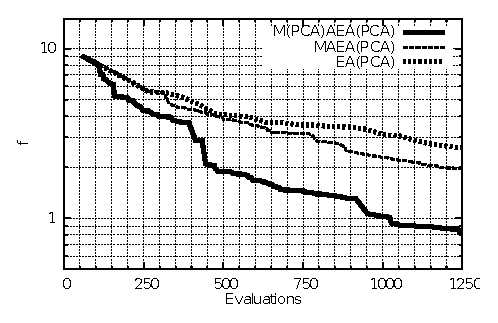
\includegraphics{1000_30d_pca_ipe.eps}}
\end{minipage}
\caption{30D non-separable ellipsoid with a=1000: Average convergence of EA(PCA), MAEA(PCA) and M(PCA)AEA(PCA). The proposed M(PCA)AEA(PCA) outperforms both of the other variants.} 
\label{Ellt3-m}
\end{figure}


Regarding the multi-dimensional and multi-modal test case of eq.\ref{mm}, a comparison regarding EA(PCA), MAEA(PCA) and M(PCA)AEA(PCA) is presented, for the 30D  problem, in fig.\ref{mmt3m}. Regarding the MAEA(PCA), the  IPE phase initiated after $300$ individuals were stored in the DB and $15$ to $19$ training patterns in the $\Re^{30}$ space were used to train the  metamodel. Regarding M(PCA)AEA(PCA), the training pattern dimension was truncated from $30$ to the $10$ most important ones with respect to f. This allowed for the  IPE phase to start just after only $100$ individuals were stored in the DB, since only $5$ to $9$ training patterns were required for the RBF network training.

\begin{figure}[h!]
\begin{minipage}[b]{1\linewidth}
 \centering
 \resizebox*{11cm}{!}{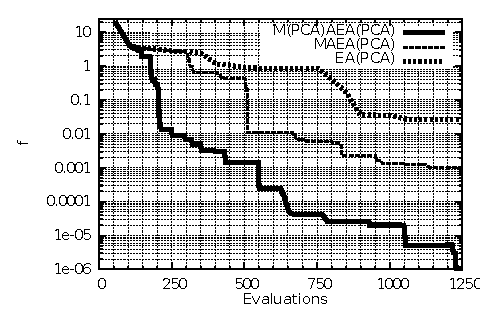
\includegraphics{30d_pca_ipe.eps}}
\end{minipage}
\caption{30D multi-modal problem: Average convergence of EA(PCA), MAEA(PCA) and M(PCA)AEA(PCA).The proposed M(PCA)AEA(PCA) method performs much better than the other variants.} 
\label{mmt3m}
\end{figure}

In figs. \ref{Ellt3-m} and \ref{mmt3m}, one may observe that the use of PCA-driven metamodels further enhances the MAEA efficiency.

%stelios

\section{Design of a Compressor Cascade}


The design of a 2D compressor cascade operating at $M_1\!=\!0.54$, $a_1\!=\!44^o$ and $Re\!=\!4\times10^5$ for minimum total pressure losses coefficient $\omega$ (eq.\ \ref{omegaLosses}) is sought. 

The blade airfoil is designed subject to a number of aerodynamic and geometrical constraints: the optimal airfoil must turn the flow by more than $30^o$ and the blade airfoil thickness at three chord-wise positions $0.3c$, $0.6c$ \& $0.9c$ must be greater that $0.10c$, $0.08c$ \& $0.01c$,  respectively.     

The airfoil shape is parameterized based on its mean-camber line and super-imposed thickness distributions, presented in section \ref{Drela1}, yielding $27$ design variables.

The advantages of using the M(PCA)AEA(PCA) method can be seen by comparing the performances of a conventional MAEA and the M(PCA)AEA(PCA). In both cases, the populations are $\mu\!=\!20$, $\lambda\!=\!60$ and $\lambda_e\!=\!6$. Both cases used local RBF networks as metamodels trained on a small number of automatically selected patterns. The MAEA used a number of  $20$ to $30$ training patterns in the $27D$ space. The IPE phase for the MAEA started after $400$ individuals were stored in the DB. Regarding M(PCA)AEA(PCA), the RBF networks used as metamodels were trained on $5$ to $8$ patterns in the  $10D$ space. The reduced dimension made the earlier use of metamodels possible; in the M(PCA)AEA(PCA) run, the IPE phase started after the first $200$ individuals were stored in the DB. 


\begin{figure}[h!]
\begin{minipage}[b]{1\linewidth}
 \centering
 \resizebox*{11cm}{!}{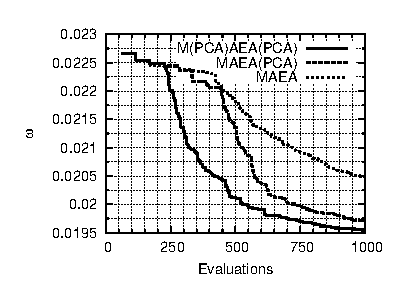
\includegraphics{CompConv_1.eps}}
\end{minipage}
\caption{Design of a compressor cascade:  Comparison of the mean value and standard deviation from  $10$ independent runs performed using MAEA, MAEA(PCA) and M(PCA)AEA(PCA).} 
\label{PCADrelaRes}
\end{figure}

Fig. \ref{PCADrelaRes} shows the convergence of both methods. M(PCA)AEA(PCA) outperforms the conventional MAEA, during all but the early generations of the optimization procedure. 

\begin{figure}[h!]
\begin{minipage}[b]{1\linewidth}
 \centering
 \resizebox*{16cm}{!}{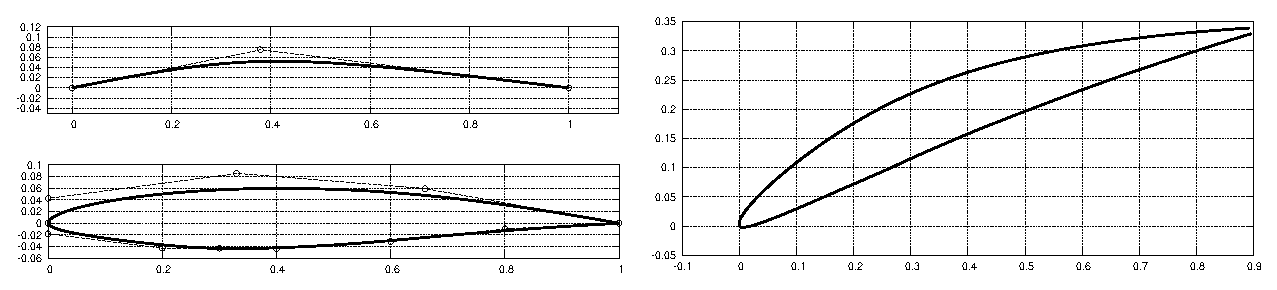
\includegraphics{ResD.eps}}
\end{minipage}
\caption{Design of a compressor cascade: The optimal airfoil resulted from M(PCA)AEA(PCA). Left: mean-camber line and thickness distribution together with their control polygons. Right: The final airfoil after superimposing thickness distributions on the mean camber line and turned to the fixed stagger angle.} 
\label{PCADrelaRes}
\end{figure}

The optimal airfoil resulting from M(PCA)AEA(PCA) run, shown in fig. \ref{PCADrelaRes}, has a total pressure loss coefficient value of $\omega=0.01803$ and respects both the thickness and flow turning constraints.  The flow turning of the optimal blade is $\Delta a=30^o$.

\begin{figure}[h!]
\begin{minipage}[b]{1\linewidth}
 \centering
 \resizebox*{10cm}{!}{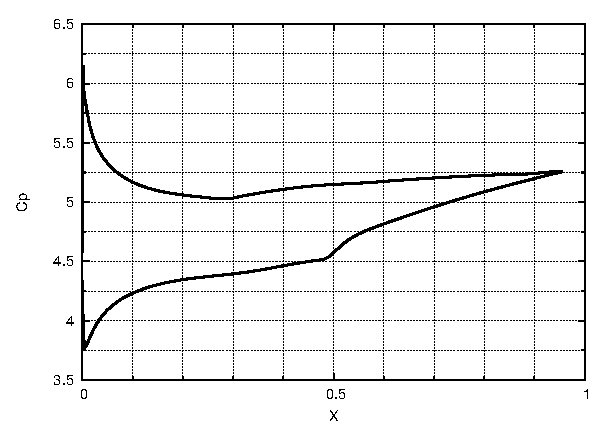
\includegraphics{Best_CP_PCA.eps}}
\end{minipage}
\caption{Design of a compressor cascade: Pressure coefficient $C_p$ of the optimal airfoil shown in fig. \ref{PCADrelaRes}.} 
\label{PCADrelaRes_cp}
\end{figure}

% ---------------------------------------------------------------------------
% ----------------------- end of thesis sub-document ------------------------
% ---------------------------------------------------------------------------